\section{Method selection and architecture}

\begin{frame}{Convolutional neural network and initial architecture}
	\begin{columns}[c]
		\begin{column}{0.55\textwidth}
			\textbf{Method selection}
			\begin{itemize}
				\item<+-> speed prediction is a \textbf{non-linear regression} task $\Rightarrow$ neural network
				\item<+-> task involves feature extraction $\Rightarrow$ \textbf{convolutional neural network} (CNN)
			\end{itemize}
			\textbf{Initial architecture}
			\begin{itemize}
				\item using paper of \textit{NVIDIA} work group \cite{NVIDIA2016} of a CNN for self-driving cars adapted on our initial data
				\item enough complexity and layers to handle the task and lots of possibilities to fine-tune it
				\item Initial results with the raw model: $\mathcal{L} < 3$ on the training set and about $\mathcal{L} = 18-20$ on the test set\\
				$\Rightarrow$ Improvements needed
			\end{itemize}
		\end{column}
		\begin{column}{0.4\textwidth}
			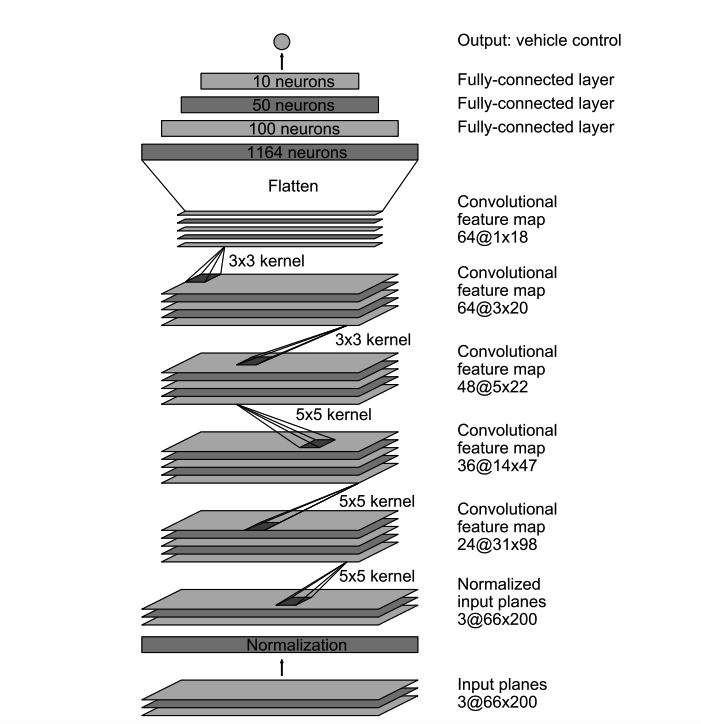
\includegraphics[width=\textwidth]{./imgs/NetworkOriginal.png}
			{\footnotesize Original architecture of the \textit{NVIDIA} paper \cite{NVIDIA2016}}
		\end{column}
	\end{columns}
\end{frame}

\begin{frame}[plain]
\begin{figure}
\centering
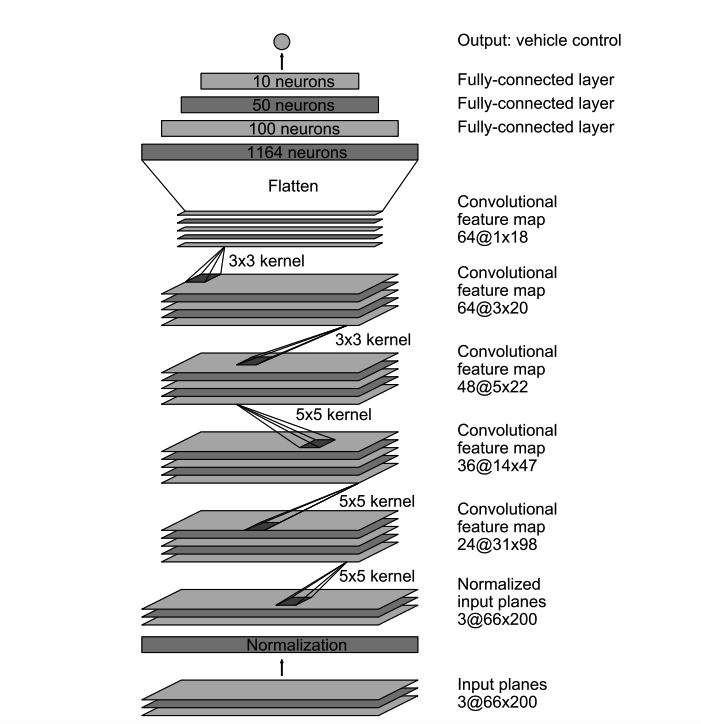
\includegraphics[scale=0.3]{./imgs/NetworkOriginal.png}
\caption{Original architecture of the NVIDIA paper \cite{NVIDIA2016}.}
\end{figure}
\end{frame}